\section{Metadata Anonymisation Toolkit (MAT)}
Metadata Anonymisation Toolkit (MAT)\footnote{ \href{https://mat.boum.org/}{https://mat.boum.org/}} wurde im Rahmen des GSoC 2011 unter Schirm�herrschaft von TorProject.org entwickelt. Es ist vor allem unter Linux einfach einsetzbar und kann folgende Datentypen s�ubern: PNG und JPEG Bilder, PDF-Dokumente, OpenOffice und Microsoft Office Dokumente, MP3 und FLAC Dateien. Das Tool ist in Python geschrieben und braucht einige Bibliotheken. Unter Debian, Ubuntu und Linux Mint installiert man zuerst die n�tigen Bibliotheken mit: 
\begin{verbatim}
 > sudo aptitude install libimage-exiftool-perl python-hachoir-core 
   python-hachoir-parser python-poppler python-cairo python-mutagen 
   python-pdfrw
\end{verbatim} 

Danach entpackt man das herunter geladene Archiv, wechselt in das neu erstellte Verzeichnis und kann das Programm starten. Es gibt eine Version f�r die Kommandozeile und eine Version mit grafischer Oberfl�che (GUI). Auf der Kommandozeile s�ubert man Dateien mit:
\begin{verbatim}
  > mat -b /path/to/datei.ext
\end{verbatim}

Die GUI-Version startet man mit:
 \begin{verbatim}
  > mat-gui
\end{verbatim}

Alternativ kann man MAT auch f�r alle User installieren mit:
\begin{verbatim}
 > sudo python setup.py install 
\end{verbatim}

In der Programmgruppe \textit{Zubeh�r} findet man den Starter f�r das GUI von MAT. Mit dem + kann man Dateien der Liste hinzuf�gen und mit dem Besen-Icon daneben s�ubern. Die ges�uberten Dateien findet im gleichen Verzeichnis, wie die Originale mit der Erweiterung \textit{.cleaned.} im Namen.

\begin{figure}[htb]
\begin{center}
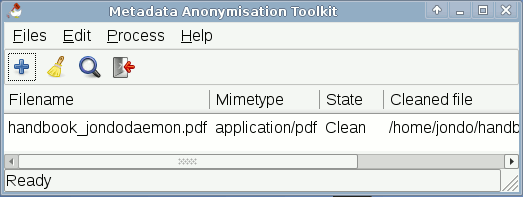
\includegraphics[scale=0.55]{../screenshots/rmmeta1.png}
\caption{Dateien s�ubern mit MAT}
\label{abb:mat}
\end{center}
\end{figure}